% Template for URSI GASS 2020 Summary Papers
%
% Use pdflatex or latex + dvips + ps2pdf to produce a PDF.
%
% 9 Dec 2016, Henrik Wallen <henrik.wallen@aalto.fi>

\documentclass[summary]{URSIGASS2020}

%% Add packages and define personal macros here, but ensure that they do not
%% interfere with the fonts and page layout. Do not add hyperlinks.

%additional defs
\def\f{\phi}
\def\o{\omega}
\def\op{\omega_{\rm p}}
\def\oH{\omega_{\rm H}}
\def\OH{\Omega_{\rm H}}
\def\Op{\Omega_{\rm p}}
\def\a{\alpha}
\newcommand{\cir}[1]{\mathop{#1}\limits^\circ}

\title{Excitation of Electromagnetic Waves by a Nonsymmetric Antenna Located on the Surface of a Semi-Infinite Gyrotropic Cylinder}

%% Use \affref{nn} and matching \aff{nn}{...} below for several authors
%% Mark the presenting author with an asterisk
\author{Oleg M. Ostafiychuk*, Vasiliy A. Es'kin, and Alexander V. Kudrin  }

%% define affiliations and addresses
\affiliation{%
  % use explicit line-breaks \\ if needed
  %\aff{ref1}{The ABC Company, Wash., DC, 20031, http://xxx.xxxx.xxx}
  %\aff{ref2}{The Next Company, Neverland, USA}
  University of Nizhny Novgorod, 23 Gagarin Ave., Nizhny Novgorod 603950, Russia
}

% (Omit \affref and \aff and the asterisk if there is only one author.)

\begin{document}

\maketitle

\begin{abstract}
Electromagnetic wave excitation by a given nonsymmetric source in the presence of a semi-infinite gyrotropic cylinder located in free space is considered.
The source-excited field and the field scattered by the end of the cylinder are represented using eigenfunction expansions that refer to the respective regions on both sides of the cylinder endface.
The distribution of the radiated power over the spatial spectrum of the excited waves is numerically analyzed.
 
\end{abstract}

\section{Introduction}

In the past decades, an enhanced attention has been paid to the problem of excitation of electromagnetic waves by given currents in systems containing open gyrotropic guiding structures.
In the case where magnetoplasma is a gyrotropic medium, such a problem arises when describing, e.g., helicon plasma sources, which are important for numerous applications [1--3].
In most studies devoted to such sources, consideration is limited to the excitation of only the discrete-spectrum waves (eigenmodes),
because they play a major role in maintaining the helicon discharge.
Many works on the subject deal with the case where an antenna is placed far from the ends of a plasma column so that it can be represented as an infinitely long guiding structure.
For such a cylindrical waveguide located in free space, the full-wave approach presented in \cite{EskinPIERS2017_meth} was applied for the analysis of the energy characteristics of a helicon-type source \cite{OstafEskin_APRASC2019}.
However, it is important in some cases to take into account a finite length of the plasma cylinder and consider diffraction by its ends \cite{Amatucci2011}.

In this work, the features of wave excitation by an antenna with the nonsymmetric electric-current distribution in the presence of a semi-infinite cylinder filled with a magnetoplasma are considered.
To find the energy characteristics of such a source, the excited field and the field scattered by the end of the cylinder are represented using eigenfunction expansions referring to the regions on both sides of the cylinder endface.

\section{Formulation of the Problem}

Consider a semi-infinite cylinder of radius $ a $ that is located in free space and has the symmetry axis coinciding with the $ z $ axis of a cylindrical coordinate system ($ \rho, \phi, z $).
The cylinder is placed in the region $ z<0 $, and its endface lies in the plane $ z=0 $, as is shown in Fig.~\ref{geometry}.
\begin{figure}[htbp]%[htbp]
	\centering
	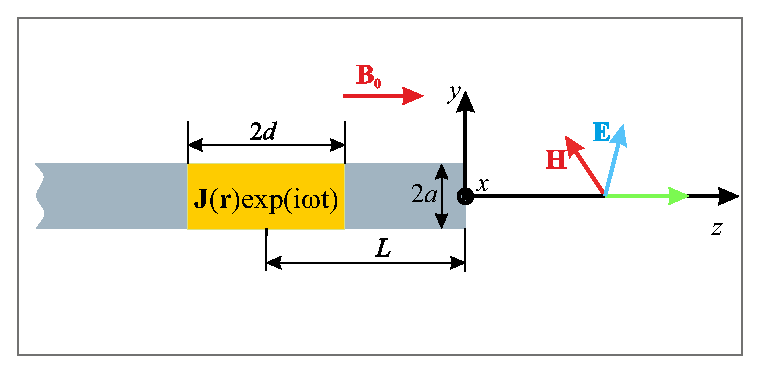
\includegraphics[width=70mm]{figures/fig1.eps}
	\caption{Geometry of the problem.}
	\label{geometry}
\end{figure}
The field is excited by an electric current specified on the side surface of the cylinder between the planes $ z=-L-d $ and $ z=-L+d $ (see Fig.~\ref{geometry}). The current density can be written, with $ \exp(i\omega t) $ time dependence dropped, as
\begin{align} \label{source_eq}
{\bf J}({\bf r})=&\,({\pmb\phi}_{0}j_{\phi}+{\bf z}_0j_z)\delta(\rho-a)
\exp\left(-im\phi-ik_0{\tilde p}z\right) \nonumber \\
&\times\left[U(z+L+d)-U(z+L-d)\right].
\end{align} 
Here, $ \delta $ is the Dirac function, $ U $ is the Heaviside function, $ d $ is the half-length of the antenna (the condition $ d<L $ is fulfilled), the integer $ m $ and the constant $ \tilde p $ determine the current dependence on the azimuthal and longitudinal coordinates, respectively, and $ k_0=\omega/c $ is the wave number in free space ($ c $  is the speed of light in free space).
The total amplitude of the current can be written as  $ |I_0|^2=|I_\phi|^2+|I_z|^2 $, where $ I_\phi=2dj_{\phi} $ and $ I_z=2\pi aj_z $.

The plasma inside the cylinder, with a superimposed static magnetic field $ \textbf{B}_{0}={B}_{0}\textbf{z}_{0} $, is described by the dielectric permittivity tensor
\begin{equation} \label{eq1}
\hat{\varepsilon}=\!\!
\left(
\begin{array}{ccc}
\varepsilon & -ig & 0 \\
ig & \varepsilon & 0 \\
0 & 0 & \eta
\end{array}
\right),
\end{equation}
where
\begin{align} \label{eq2}
&\varepsilon =\!1+\frac{\op^2}{\oH^2-\omega^2}+\frac{\Op^2}{\OH^2-\omega^2}, \quad
\eta=1-\frac{\op^2}{\omega^2}-\frac{\Op^2}{\omega^2},
 \nonumber \\
&\hspace{10mm}g=-\frac{\op^2\oH}{(\oH^2-\omega^2)\omega}+\frac{\Op^2\OH}{(\OH^2-\omega^2)\omega}.
\end{align}
Here, $ \op $ and $ \Op $ are the electron and ion plasma frequencies, and $ \oH $ and $ \OH $ are the gyrofrequencies of the corresponding particles, respectively.
Note that the Gaussian system of units is used throughout this work.

\section{The Source-Excited and Diffracted Fields}

Using the cylindrical symmetry of the problem, the longitudinal components of the excited and diffracted fields can be represented as 
\begin{equation}\label{modal_fields}
\begin{bmatrix} {E}_{z;s,m}({\bf r},q)\\ {	H}_{z;s,m}({\bf r},q)\end{bmatrix} = \begin{bmatrix} {E}_{z;s,m}(\rho, q)\\ {H}_{z;s,m}(\rho, q)\end{bmatrix}e^{-i m\f - i k_0
	p_{s}(q)z}.
\end{equation}
Here, the azimuthal index $ m $ is the same as in (\ref{source_eq}), the subscript $ s $  denotes the wave propagation direction, either positive ($ s=+ $) or negative ($ s=- $), and $ q $ and $p_{s}(q)$ are the normalized (to $ k_{0} $) transverse and longitudinal wave numbers in free space, respectively.
The function $ p_{s}(q) $ obeys the relation $p_{\rm +}(q)\equiv p(q)= -p_{\rm -}(q)$, where $ p(q)=(1-q^2)^{1/2} $.
It is assumed that $ {\rm Re}[p(q)]>0 $ if $ q $ is real and less than unity, and  $ {\rm Im}[p(q)]<0 $ otherwise.
The transverse field components  $E_{\rho;s,m}$, $E_{\f;s,m}$, $H_{\rho;s,m}$, and $H_{\f;s,m}$ can be found from the longitudinal components (\ref{modal_fields}).
In what follows, we take into account that only the waves with the azimuthal index $ m $ are excited by the source.

The field excited by the given current (\ref{source_eq}) in the half-space $ z<0 $ is expanded in terms of eigenwaves of an open waveguide and is written in the source-free regions as
\begin{align}\label{eq4} 
&\hspace{-4mm}\left[\!\!\!
\begin{array}{c}
{E_z^{(\rm ex)}}({\bf r})\\
{H_z^{(\rm ex)}}({\bf r})
\end{array}\!\!\!\right] = 
\sum_{n}a_{s,m,n}
\left[\!\!\!
\begin{array}{c}
{E}_{z;s,m,n}(\rho)\\
{H}_{z;s,m,n}(\rho)
\end{array}\!\!\!\right]e^{-im\f - ik_0 p_{s,m,n}z} \nonumber\\ 
&\hspace{0mm}+\sum_{\alpha=1}^2\,\int_{0}^{\infty}\!\!\!a_{s,m,\alpha}(q)
\left[\!\!\!
\begin{array}{c}
{E}_{z;s,m,\alpha}(\rho,q)\\
{H}_{z;s,m,\alpha}(\rho,q)
\end{array}\!\!\!\right]e^{-im\f - ik_0 p_{s} z}dq.
\end{align}
Here, $ s=+ $ for $ -L+d<z<0 $ and $ s=- $ for $ z<-L-d $; the functions $ E_{z;s,m,n}(\rho) $ and $ H_{z;s,m,n}(\rho) $ describe the radial distributions of the fields of the discrete-spectrum waves (eigenmodes) with the radial index $ n $ and the longitudinal wave numbers $ p_{s,m,n} $ ($ p_{+,m,n}=-p_{-,m,n}=p_{m,n} $);
and the subscript $ \alpha $ corresponds to two kinds of the continuous-spectrum waves described by the functions $ E_{z;s,m,\alpha}(\rho,q) $ and $ H_{z;s,m,\alpha}(\rho,q) $.
Detailed expressions for these fields, which constitute the complete set of eigenwaves of an open gyrotropic cylindrical waveguide, can be found in \cite{EskinPIERS2017_meth}.
The quantities $ a_{s,m,n} $ and $ a_{s,m,\alpha}(q) $ are obtained using the well-known technique developed for finding the expansion coefficients of the modes of open waveguides \cite{Kondrat'ev1999} and are given by the expressions
\begin{align}\label{eq5}
a_{s,m,n}=&\frac{1}{N_{+,m,n}} \int{\bf J}({\bf r})\cdot{\bf E}^{({\rm T})}_{-s,-m,n}({\bf r})d{\bf r} \nonumber\\
=&\left[j_{\phi}{E}^{({\rm T})}_{\phi;-s,-m,n}(a) + j_z {E}^{({\rm T})}_{z;-s,-m,n}(a)\right] \nonumber \\
&\times\frac{4\pi a}{N_{+,m,n}}\frac{\sin\left[k_0(\tilde{p} - p_{s,m,n})d\right]}{k_0(\tilde{p} - p_{s,m,n})}e^{-ik_0p_{s,m,n}L}, \nonumber\\
a_{s,m,\alpha}(q)=&\frac{1}{N_{+,m,\alpha}(q)} \int{\bf J}({\bf r})\cdot{\bf E}^{({\rm T})}_{-s,-m,\alpha}({\bf r},q)d{\bf r} \nonumber \\
=&\left[j_{\phi}{E}^{({\rm T})}_{\phi;-s,-m,\alpha}(a,q) + j_z {E}^{({\rm T})}_{z;-s,-m,\alpha}(a,q)\right] \nonumber \\
&\times\frac{4\pi a}{N_{+,m,\alpha}(q)} \frac{\sin\left[k_0(\tilde{p} - p_s(q))d\right]}{k_0(\tilde{p} - p_s(q))}e^{-ik_0p_{s}L}, 
\end{align}
where integration is performed over the region occupied by the current (\ref{source_eq}), the superscript (T) denotes fields taken in an auxiliary medium that is described by the transposed dielectric permittivity tensor ${\hat{\varepsilon}}^{\rm T}$, and $ N_{s,m,n} $ and $ N_{s,m,\alpha}(q) $ are the norms of the discrete- and continuous-spectrum waves, respectively, which follow from the orthogonality relations presented in \cite{EskinPIERS2017_meth}.

The field reflected from the cylinder end to the region $ z<0 $ is also expanded in terms of eigenwaves of an open gyrotropic waveguide.
The longitudinal components of the reflected field, hereafter marked by the superscript ($ \rm r $), are represented as
\begin{align}\label{eq6}
&\hspace{-4mm}\left[\!\!\!
\begin{array}{c}
{E_z^{(\rm r)}}({\bf r})\\
{H_z^{(\rm r)}}({\bf r})
\end{array}\!\!\!\right]\!\!{=}\!\sum\limits_{n} b_{-,m,n}\!\!\left[\!\!\!
\begin{array}{c}
{E}_{z;-,m,n}(\rho)\\
{H}_{z;-,m,n}(\rho)
\end{array}\!\!\!\right]\!\!e^{-im\f + ik_0 p_{m,n}z}\notag\\
&+ \sum\limits_{\alpha=1}^{2}\int_{0}^{\infty}\!\!\!b_{-,m,\alpha}(q)\!\!\left[\!\!\!
\begin{array}{c}
{E}_{z;-,m,\alpha}(\rho,q)\\
{H}_{z;-,m,\alpha}(\rho,q)
\end{array}\!\!\!\right]\!\!e^{-im\f + ik_0 p z}\,dq,
\end{align}
where $ b_{-,m,n} $ and $ b_{-,m,\alpha}(q) $ are the expansion coefficients to be found.

The field transmitted to the region $ z>0 $ is expanded in terms of the continuous-spectrum waves of free space as
\begin{align}\label{eq7}
&\hspace{-2mm}\left[\!\!\!\!
\begin{array}{c}
{E_z^{(\rm t)}}\\
{H_z^{(\rm t)}}
\end{array}\!\!\!\!\right]\!
{=}\!\sum\limits_{\gamma=1}^{2}\!\int_{0}^{\infty}\!\!\!\!\!\!\! c_{+,m,\gamma}(q)\!\!\left[\!\!\!
\begin{array}{c}
E_{z;+,m,\gamma}(\rho,q)\\
H_{z;+,m,\gamma}(\rho,q)
\end{array}\!\!\!\right]\!\!e^{-i m\f-ik_0 p z}{d}q,
\end{align}
where the superscript~$({\rm t})$ denotes the field transmitted to free space, $\gamma=1$ and $\gamma=2$ correspond to the $E$- and $H$-polarized waves, respectively, and $ c_{+,m,\gamma}(q) $ are unknown coefficients depending on $ q $.
The eigenwaves of free space are written as
\begin{align}\label{eq8}
E_{z;s,m,\gamma}(\rho,q) {=} q J_m(k_0q \rho)\delta_{\gamma,1},\nonumber\\ H_{z;s,m,\gamma}(\rho,q) {=} q J_m(k_0q \rho)\delta_{\gamma,2},
\end{align}
where $J_m$ is the Bessel function of the first kind of order $m$ and $\delta_{\rm
\alpha,\beta}$ is the Kronecker delta.

Satisfying the boundary conditions for the tangential field components at the plane $ z=0 $, i.e.,
\begin{eqnarray}\label{bound_cond}
&&\hspace{-5mm}{E}^{(\rm ex)}_{\rho}+{E}^{(\rm r)}_{\rho}={E}^{(\rm t)}_{\rho},\quad {E}^{(\rm ex)}_{\f}+{E}^{(\rm r)}_{\f}={E}^{(\rm t)}_{\f},\nonumber\\
&&\hspace{-5mm}{H}^{(\rm ex)}_{\rho}+{H}^{(\rm r)}_{\rho}={H}^{(\rm t)}_{\rho},\quad {H}^{(\rm ex)}_{\f}+{H}^{(\rm r)}_{\f}={H}^{(\rm t)}_{\f},
\end{eqnarray}
and taking into account the orthogonality relations for the eigenwaves in the regions $ z<0 $ and $ z>0 $, a system of integral equations for the expansion coefficients $ b_{-,m,n} $, $ b_{-,m,\alpha}(q) $, and $ c_{+,m,\gamma}(q) $ is derived in the following form:
\begin{align}
&c_{+,m,\gamma}(q)\tilde{N}_{+,m,\gamma}(q)=\sum_{n}a_{+,m,n}K_{-,-m,\gamma}^{+,m,n}(q) \nonumber\\
&+ \sum_{\alpha=1}^{2}\int_{0}^{\infty}\!\!\!a_{+,m,\alpha}(\tilde{q})K_{-,-m,\gamma}^{+,m,\alpha}(\tilde{q},q)d\tilde{q} \nonumber+\sum_{n}b_{-,m,n}K_{-,-m,\gamma}^{-,m,n}(q) \\
&+\sum_{\alpha=1}^{2}\int_{0}^{\infty}\!\!\!b_{-,m,\alpha}(\tilde{q})K_{-,-m,\gamma}^{-,m,\alpha}(\tilde{q},q)d\tilde{q}, \label{int_eq1} \\ 
&b_{-,m,n}N_{-,m,n}=\sum_{\gamma=1}^{2}\int_{0}^{\infty}\!\!\!\!c_{+,m,\gamma}(\tilde{q})M_{+,m,\gamma}^{+,-m,n}(\tilde{q})d\tilde{q}, \label{int_eq2} \\
&b_{-,m,\alpha}({q})N_{-,m,\alpha}({q})\!=\!\!\!\sum_{\gamma=1}^{2}\!\int_{0}^{\infty}\!\!\!\!\!\!\!c_{+,m,\gamma}(\tilde{q})M_{+,m,\gamma}^{+,-m,\alpha}(q,\tilde{q})d\tilde{q}. \label{int_eq3}
\end{align}
The norm of the eigenwaves of free space in \eqref{int_eq1} is given by the formula
\begin{equation}\label{norm_free_space}
\hspace{-7mm} {\tilde N}_{s,m,{\gamma}}({q})=(-1)^{m+\gamma}{c}{p_s}/({k_0^2}{q}),
\end{equation}
and the kernels of integral equations (\ref{int_eq1})--(\ref{int_eq3}) are written as
\begin{align}
&K_{-,-m,\gamma}^{s,m,n}(q)\!=\!\frac{c}{4\pi}\int_{0}^{2\pi}\!\!\!\!\!{d}{\phi}\!\!\!\!\int_{0}^{\infty}\!\!\left[{\bf E}_{s,m,{n}}({\bf r}){\times}{\bf H}_{-,-m,\gamma}({\bf r},{q})\right.\nonumber\\
&\hspace{19mm}\left. - {\bf E}_{-,-{m},\gamma}({\bf r},{q}){\times}{\bf H}_{s,m,{n}}({\bf r})\right]\!\!{\cdot}{\bf z}_0\rho{d}\rho,\nonumber\\
&K_{-,-m,\gamma}^{s,m,\a}(\tilde{q},q)\!=\!\frac{c}{4\pi}\int_{0}^{2\pi}\!\!\!\!\!{d}{\phi}\!\!\!\!\int_{0}^{\infty}\!\!\left[{\bf E}_{s,m,{\a}}({\bf r},\tilde{q}){\times}{\bf H}_{-,-m,\gamma}({\bf r},{q})\right.\nonumber\\
&\hspace{22mm}\left. - {\bf E}_{-,-{m},\gamma}({\bf r},{q}){\times}{\bf H}_{s,m,{\a}}({\bf r},\tilde{q})\right]\!\!{\cdot}{\bf z}_0\rho{d}\rho,\nonumber\\
&M_{+,m,\gamma}^{+,-m,n}(\tilde{q})\!=\!\frac{c}{4\pi}\int_{0}^{2\pi}\!\!\!\!\!{d}{\phi}\!\!\!\!\int_{0}^{\infty}\!\!\left[{\bf E}_{+,m,{\gamma}}({\bf r},\tilde{q}){\times}{\bf H}^{({\rm T})}_{+,-m,n}({\bf r})\right.\nonumber\\
&\hspace{20mm}\left. - {\bf E}^{({\rm T})}_{+,-{m},n}({\bf r}){\times}{\bf H}_{+,m,{\gamma}}({\bf r},\tilde{q})\right]\!\!{\cdot}{\bf z}_0\rho{d}\rho,\nonumber\\
&M_{+,m,\gamma}^{+,-m,\alpha}(q,\tilde{q})\!=\!\frac{c}{4\pi}\int_{0}^{2\pi}\!\!\!\!\!{d}{\phi}\!\!\!\!\int_{0}^{\infty}\!\!\left[{\bf E}_{+,m,{\gamma}}({\bf r},\tilde{q}){\times}{\bf H}^{({\rm T})}_{+,-m,\alpha}({\bf r},q)\right.\nonumber\\
&\hspace{23mm}\left. - {\bf E}^{({\rm T})}_{+,-{m},\alpha}({\bf r},\tilde{q}){\times}{\bf H}_{+,m,{\gamma}}({\bf r},q)\right]\!\!{\cdot}{\bf z}_0\rho{d}\rho. \label{eq14}
\end{align}
The power carried through the cross section $ z = z_{0}<-L-d $ to the negative direction of the $ z $-axis is determined by the expansion coefficients of the source-excited and reflected fields as $ P^{(-)}=P_{\rm mod}+P_{\rm cs} $, where
\begin{align}
P_{\rm mod}=&\sum_{n}P_{n}=\sum_{n}|a_{-,m,n}+b_{-,m,n}|^2{\cal P}_{+,m,n} \label{P_mod}
\end{align}
describes the contribution of the discrete-spectrum waves
($ P_{n} $ is the partial power going to the $ n $th eigenmode), whereas
\begin{align}
P_{\rm cs}=&\sum_{\alpha=1}^{2}\int_{0}^{1}|a_{-,m,\a}(q)+b_{-,m,\a}(q)|^2{\cal P}_{+,m,\a}(q)dq \label{P_cs}
\end{align}
describes the contribution of the continuous-spectrum waves. Here, $ {\cal P}_{s,m,n} $ and $ {\cal P}_{s,m,\alpha} $ are defined by the power orthogonality relations presented in \cite{OstafEskin_APRASC2019}.
In deriving \eqref{P_mod} and \eqref{P_cs}, the relations $ {\cal P}_{+,m,n}=-{\cal P}_{-,m,n} $ and $ {\cal P}_{+,m,\alpha}(q)=-{\cal P}_{-,m,\alpha}(q) $ were used.
The power transmitted from the cylinder end to the region $ z>0 $ is expressed via the expansion coefficients for waves in free space as
\begin{equation}\label{forward_powers}
P^{(+)}=\sum_{\gamma=1}^{2}\int_{0}^{1}|c_{+,m,\gamma}(q)|^2\frac{cp(q)}{4k_{0}^{2}q}dq.
\end{equation}

\section{Numerical results}
Integral equations \eqref{int_eq1}--\eqref{int_eq3} were numerically solved using Simpson's integration method.
The powers going to the eigenwaves of the cylinder and free space have been calculated for the parameters $ a=2{.}5 $\,cm, $ d=4a $, $ {\tilde p}=0 $, and $ m=1 $, which are typical of helical antennas used in helicon plasma devices.
It is assumed that the frequency of the source belongs to the resonant interval $ \omega_{\rm LH}<\omega<\oH $ of the whistler range, where $ \omega_{\rm LH}=(\oH\OH)^{1/2} $ is the lower-hybrid frequency.
The following values of the dimensionless parameters of the plasma were used for calculations: $\o_{p}/\o_{H} = 12{.}7$, $  \omega_{\rm LH}/\oH=3{.}7\times10^{-3} $, and  $\o_{H} a/c = 1{.}17$.
Note that due to the fact that a magnetoplasma is resonant in the considered frequency range, the cylinder supports an infinite number of the propagating eigenmodes.
Figure~\ref{fig_P_from_L} shows the powers $ P_{\rm mod} $ and $ P_{\rm cs} $ as functions of $ L $ that varies in the range $ 5a<L<2\lambda_{0} $ ($ \lambda_{0}=2\pi/k_{0}\gg a$ is the free-space wavelength). All the values presented in this and the forthcoming figures are normalized to the total power $ P_{0} $ radiated from the same source in the case where the cylinder is infinite. 
\begin{figure}[!b]
	\centering
	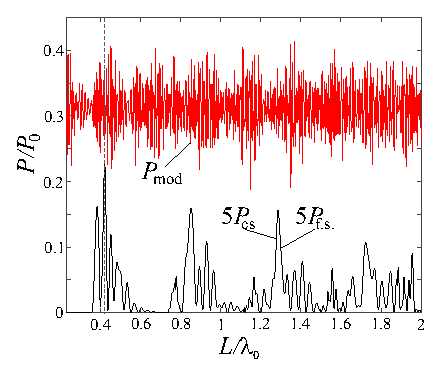
\includegraphics[width=73mm]{figures/fig_P_from_L.eps}
	\caption{The normalized powers $ P_{\rm mod} $ (red line) and $ P_{\rm cs} $ (black line) as functions of the parameter $ L/\lambda_{0} $ for $  \omega/\oH=2{.}5\times10^{-2} $, $\o_{p}/\o_{H} = 12{.}7$, $  \omega_{\rm LH}/\oH=3{.}7\times10^{-3} $, $\o_{H} a/c = 1{.}17$, and $ j_z=0{.}25 j_{\f} $. The value of $ P_{\rm cs} $ is multiplied by $ 5 $.}
	\label{fig_P_from_L}
\end{figure}
It is seen in Fig.~\ref{fig_P_from_L} that the inequality $ P_{\rm mod}\gg P_{\rm cs} $ holds for the chosen parameters.
The power $ P_{\rm cs} $ carried by the continuous-spectrum waves increases notably at certain values of $ L/\lambda_{0} $, remaining to be less than $ P_{\rm mod} $.
As was shown by the calculations, the relation $ P^{(+)} \simeq P_{\rm cs} $ is valid for the power going to the region $ z>0 $ for each value of $ L $.
Thus, the most of the radiated power goes to the discrete-spectrum waves. Those of them that propagate in the positive $ z $-axis direction are almost entirely reflected from the cylinder end.
Note that the total radiated power $ P_{\Sigma}=P_{\rm mod}+ P_{\rm cs}+P^{(+)}  $ can change with varying $ L $ because of the interference of the excited and reflected waves.

The partial powers $P_n$ going to the discrete-spectrum waves (for the first $ 75 $ eigenmodes for which $ p_{n}<200 $) are shown in Figs.~\ref{fig_P_mod}(a) and \ref{fig_P_mod}(b) for two values of $ L/\lambda_{0} $.
\begin{figure}[tbp]
	\centering
	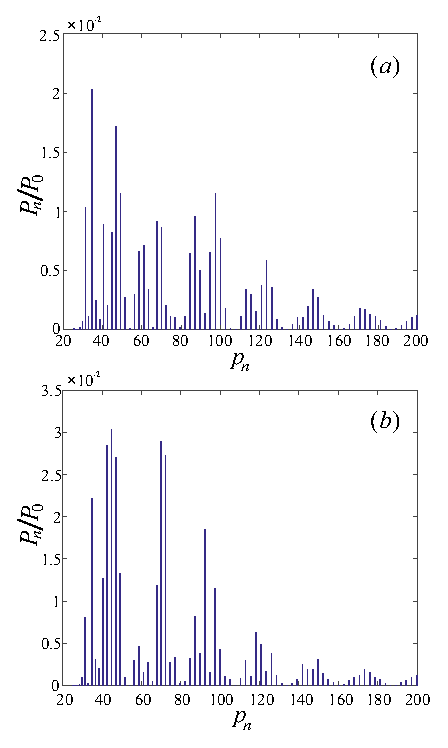
\includegraphics[width=73mm]{figures/fig_P_mod.eps}
	\caption{The normalized partial powers $P_n$ for the individual eigenmodes with the radial indices $ n $ and the longitudinal wave numbers $ p_n $ for $ L=0{.}423\lambda_{0} $ (a) and $ L=0{.}697\lambda_{0} $ (b). Same parameters as in Fig.~\ref{fig_P_from_L}.}
	\label{fig_P_mod}
\end{figure}
In the case presented in Fig.~\ref{fig_P_mod}(a), the ratio of the powers going to the discrete- and continuous-spectrum waves amounts to its minimum value $ P_{\rm mod}/(P_{\rm cs}+P^{(+)})\simeq3 $ at $ L=0{.}423\lambda_{0} $.
The corresponding value of $ L/\lambda_{0} $ is indicated by the vertical dashed line in Fig.~\ref{fig_P_from_L}.
The ratio of the powers changes periodically with increasing $ L $ and reaches one of its maximum values $ P_{\rm mod}/(P_{\rm cs}+P^{(+)})\simeq2\times10^{3} $ at $ L=0{.}697\lambda_{0} $.
In this case, the quantities $P_n$ are presented in Fig.~\ref{fig_P_mod}(b).
It follows from comparison of Figs.~\ref{fig_P_mod}(a) and \ref{fig_P_mod}(b) that a notable redistribution of the partial powers over the spatial spectrum occurs when the parameter $ L/\lambda_{0} $ varies.

{\enlargethispage{-0.12in}}

\section{Conclusions}
In this work, the electromagnetic wave excitation has been studied in the case where the nonsymmetric given source is placed on the surface of a semi-infinite cylinder filled with a magnetoplasma.
The integral equations for the field expansion coefficients of the waves diffracted by the end of the cylinder have been derived and numerically solved.
The partial powers going to the discrete- and continuous-spectrum waves as functions of the distance from the antenna to the cylinder end have been analyzed. 
It has been demonstrated that in the whistler frequency range, almost all the radiated power goes to the eigenmodes, which are then reflected from the cylinder end.
It has also been established that the distribution of the radiated power over the spatial spectrum of excited waves noticeably depends on the source position.

\section{Acknowledgements}

This work was supported by the Russian Science Foundation (project No.~18--72--10046).

\begin{thebibliography}{99}
\bibitem{Chen_review_2015} F. F. Chen, ``Helicon Discharges and Sources: A Review,'' \emph{Plasma Sources Science and Technology}, \textbf{24}, p.~014001, January 2015, doi: 10.1088/0963-0252/24/1/014001.

\bibitem{Caneses_Blackwell} J.\,F.~Caneses, B.\,D.~Blackwell, and P.~Piotrowicz, ``Helicon Antenna Radiation Patterns in a High-Density Hydrogen Linear Plasma Device,'' \emph{Physics of Plasmas}, \textbf{24}, 11, November 2017, p.~113513, doi: 10.1063/1.5000848.

\bibitem{Amatucci2011}
W.\,E.~Amatucci, D.\,D.~Blackwell, E.\,M.~Tejero, C.\,D.~Cothran, L.\,Rudakov, G.\,I.~Ganguli, and D.\,N.~Walker, ``Whistler Wave Resonances in Laboratory Plasma,'' \emph{IEEE Transactions on Plasma Science}, \textbf{39}, 2, February 2011, pp.~637--643, doi: 10.1109/TPS.2010.2096235.

\bibitem{EskinPIERS2017_meth} V.\,A.~Es'kin and A.\,V.~Kudrin, ``A New Method for Con\-structing an Orthogonal System of Eigenwaves of an Open Cylindrical Waveguide Surrounded by an Isotropic Medium,'' \emph{Proceedings of PIERS 2017}, May 2017, pp.~843--848, doi: 10.1109/PIERS.2017.8261860.

\bibitem{OstafEskin_APRASC2019} O.\,M.\,Ostafiychuk, V. A. Es'kin, and A. V. Kudrin, ``Electromagnetic Wave Excitation by a Nonsymmetric Antenna Located on the Surface of an Open Gyrotropic Cylindrical Waveguide,'' \emph{Proceedings of 2019 URSI AP-RASC}, March 2019, pp. 1--4, doi:  10.23919/URSIAP-RASC.2019.8738518.
	
\bibitem{Kondrat'ev1999} I.\,G.~Kondrat'ev, A.\,V.~Kudrin, and T.\,M.\,Za\-bo\-ron\-ko\-va,
\emph{Electrodynamics of Density Ducts in Magnetized Plasmas}, Amsterdam: Gordon and
Breach, 1999.
	
\end{thebibliography}


\end{document}
